\chapter{Theorie und Grundlagen}
\label{ch:theorybasics}
\section{\textcolor{red}{Signifikanz von Kartendaten}}
% Kartendaten Decken alles ab\\
% Parks, Points of Interests etc.\\
% Ansichten für Satellit und Map\\
% ÖPNV von Bus/Tram bis zu internationalen Zügen\\

\section{\textcolor{red}{Verwendung von Indoor Maps}}
% Einkaufszentren, Stadien, Flughäfen, Bahnhöfen

\section{Zeichnen auf Kartendaten}
Indoor Maps beschreiben in erster Linie die Positionen, Strukturen und Funktionsweisen von Räumlichkeiten in Gebäuden. Diese Informationen, die auf Kartendaten gezeichnet werden müssen, lassen sich mit Hilfe der \acs{geojson} beschreiben. Dabei muss beachtet werden, dass man die Syntax des Formats einhält.

\subsection{Das JSON-Format}
Die \ac{json} ist ein textbasiertes und sprachenunabhängiges Datenaustauschformat, welches Informationen strukturiert darstellen kann. Dabei ist ein großer Vorteil gegenüber anderen Datenaustauschformaten, dass \ac{json} für sowohl Mensch als auch Maschine einfach zu lesen ist und zudem die enthaltenen Informationen auf ein benötigtes minimum reduziert. Gerade durch die für Maschinen einfach zu interpretierende Struktur lassen sich \ac{json}-Inhalte schneller parsen und verarbeiten \parencite{WYS2014}. Der Standard wird von der Internet Engineering Task Force\footnote{RFC 8259} und der European Computer Manufacturers Association (ECMA) spezifiziert\footnote{ECMA-404}.\pbreak%
%
Der Kern von \ac{json} besteht aus den sogenannten Objekten, die Key-Value-Paare enthalten. Dabei ist ein Key immer vom Typ \texttt{string} und ein Value vom Typ \texttt{object}, \texttt{array}, \texttt{string}, \texttt{number}, \texttt{boolean} oder \texttt{null}. Ein Array kann aus den selben Typen bestehen wie der Wert eines Key, sodass sich auch Objekte und Arrays verschachteln lassen können. Dabei ist zu beachten, dass gültiges \ac{json} entweder mit einem Objekt oder einem Array beginnt. Im Listing \ref{lst:jsonexample} kann man ein \ac{json}-Konstrukt sehen, bestehend aus einem Array, welches mehrere Objekte mit Keys enthalten kann, die eine Person beschreiben, wie \texttt{name}, \texttt{age} und \texttt{parents}. %
Das \texttt{parents}-Array kann wieder Objekte beinhalten, die eine Person beschreiben.
\codelisting{Beispielcode eines JSON-Konstrukts}{lst:jsonexample}{json-example.json}{json}%
%
\subsection{Das GeoJSON-Format}
Bei der \ac{geojson} handelt es sich um ein Datenaustauschformat, welches auf \ac{json} basiert und sich an der Syntax von \ac{json} orientiert. Der Standard wurde Anfang 2007 begonnen und Mitte 2008 als GeoJSON Specification veröffentlicht. In 2015 wurde eine neue GeoJSON Working Group von der Internet Engineering Task Force gegründet, die den Standard nun spezifiziert\footnote{RFC 7948}. Die veraltete GeoJSON Specification wurde daher für obsolet erklärt und wird nicht mehr verwendet \parencite{BUT2008}.\pbreak%
%
Für die Darstellung von Geometrien werden sogenannte \textit{Features} erstellt, die eine \textit{Geometry} und \textit{Properties} haben. In der Geometry werden die Koordinaten und der Typ der Geometrie angegeben, während man in den Properties die Möglichkeit hat beliebige weitere Daten zu hinterlegen. Die \ac{geojson}-Spezifikation bietet sechs verschiedene Geometrie-Typen an, die die angegebenen Koordinaten unterschiedlich verarbeiten. Diese sind \texttt{Point}, \texttt{LineString}, \texttt{Polygon}, \texttt{MultiPoint}, \texttt{MultiLineString} und \texttt{MultiPolygon}.
\codelisting{Beispielcode eines GeoJSON-Features}{lst:geojsonfeature}{geojson-feature-example.geojson}{json}\pbreak
Möchte man Features gruppieren, kann man diese in eine \texttt{FeatureCollection} ablegen. Eine FeatureCollection hat keine weiteren Eigenschaften wie einen Namen, sie gruppiert lediglich mehrere Features.
\codelisting{Beispielcode einer GeoJSON-FeatureCollection}{lst:geojsonfeaturecol}{geojson-featurecol-example.geojson}{json}

\subsection{Indoor Mapping Data Format}
Das \ac{imdf} ist ein gebündeltes Format bestehend aus 16 \ac{geojson} und einer \ac{json}-Datei. Die Spezifikation wurde erstmals 2019 auf der World Wide Developer Conference vorgestellt \parencite{GOD2019} und seitdem weiterentwickelt. In der Spezifikation beschreibt sich das Format selbst mit den Worten \blockquote{[...][IMDF] provides a generalized, yet comprehensive model for any indoor location, providing a basis for orientation, navigation and discovery.} \parencite{HOA2019}\pbreak%
%
Für diesen Zweck stellt das \ac{imdf} 16 verschiedene \textit{FeatureTypes} zur Verfügung. Ein \ac{imdf}-Feature ist ein Superset eines \ac{geojson}-Features und erweitert die Spezifikation um zwei Eigenschaften: Die \texttt{id}, welche ein \ac{uuid} ist und das Feature im gesamten \ac{imdf}-Projekt eindeutig identifiziert, sowie der \texttt{feature\_type}, welcher die Typbezeichnung für das aktuelle Feature enthält.
Die Typen unterscheiden sich in erster Linie in ihrer Aufgabe, ihrer Geometry und ihren Properties. Ein Footprint-Feature muss zum Beispiel immer ein Polygon oder MultiPolygon sein und die Properties \texttt{category}, \texttt{name} und \texttt{building\_ids} haben, während ein Address-Feature andere Properties und keine Geometry hat.\pbreak%
%
Über Verweise der \ac{uuid}s einzelner Features lassen sich so Abhängigkeiten erzeugen, die den Aufbau der Indoor Map beschreiben. Ein Raum ist einer Etage zugeordnet, die Etage kann in mehreren Gebäuden vorkommen und jedes dieser Gebäude kann eine Adresse haben.

\section{Typen mobiler Anwendungen}
Wenn es um die Entwicklung mobiler Anwendungen geht, gibt es mehrere Möglichkeiten und jede dieser Möglichkeiten hat Vor- sowie Nachteile in unterschiedlichen Bereichen.
Die Entscheidung, welcher Typ sinnvoll ist, ist sehr anwendungsspezifisch.
Aus diesem Grund müssen die Vor- und Nachteile gegeneinander abgewägt werden.
Für welchen Typ von mobilen Anwendung sich entschieden wurde, wird am Ende begründet.

\subsection{Native Anwendungen}
Wenn eine mobile Anwendung für eine bestimmte Plattform entwickelt werden soll, nutzt man die nativen Programmiersprachen und sogenannte \Glspl{sdk} der Hersteller.
Native Anwendungen haben einen direkten Zugriff auf die Schnittstellen der Gerätehersteller und werden nativ auf dem Gerät ausgeführt.
Für Android-Geräte werden unter anderem die Programmiersprachen \textit{Java} und \textit{Kotlin} verwendet, während man bei Apple Geräten mit den Programmiersprachen \textit{Objective-C} oder \textit{Swift} entwickeln kann.
Der größte Vorteil gegenüber den anderen Typen ist die Leistung und Stabilität der Anwendungen.
Die Anwendungen werden für die Zielplatform entwickelt und müssen sich daher nur auf diese konzentrieren.
Ein signifikanter Nachteil besteht darin, dass man mit einer nativen Anwendung nur ein Betriebssystem bedient und mehrere Codebasen benötigen würden, wenn man alle bekannten Betriebssysteme unterstützen möchte.

\subsection{Webbasierte Anwendungen}
Im Gegensatz zu nativen mobilen Anwendungen kann man mit einer webbasierten Anwendung die Benutzer aller Betriebssysteme ansprechen – sofern ein Webbrowser vorhanden ist.
Es muss nur eine Codebasis verwaltet werden und die Anwendung wird mit Webtechnologien entwickelt.
Unterschiedliche Webbrowser können auch unterschiedliche Funktionalitäten haben oder Inhalte anders darstellen.
Das liegt daran, dass die Hersteller der Webbrowser die erarbeiteten Standards unterschiedliche interpretieren und implementieren \parencite{RED2016}.
Kaum Unterschiede in der Anzeige der Inhalte gibt es bei den Webbrowsern \textit{Chrome} von Google und \textit{Safari} von Apple, da beide auf der HTML-Rendering-Engine \textit{WebKit} basieren \parencite{PIC2008}. Seit 2013 nutzt Google die HTML-Rendering-Engine \textit{Blink} - eine Abspaltung von WebKit – für ihren Browser und entwickelt diese weiter \parencite{BAR2013}. Erkennbar in der Abbildung \ref{fig:browser-market-share} erreichen die beiden größten Vertreter der mobilen Webbrowser zusammen \SI{84.1}{\prc} aller Nutzer \parencite{STA2020}.
Mit kleinen Anpassungen am Code oder der Einbindung von bestimmten \Glspl{library} kann man dafür sorgen, dass eine webbasierte Anwendung in allen Webbrowsern gleich funktioniert und noch mehr Nutzer erreichen.
\begin{figure}[h!]
	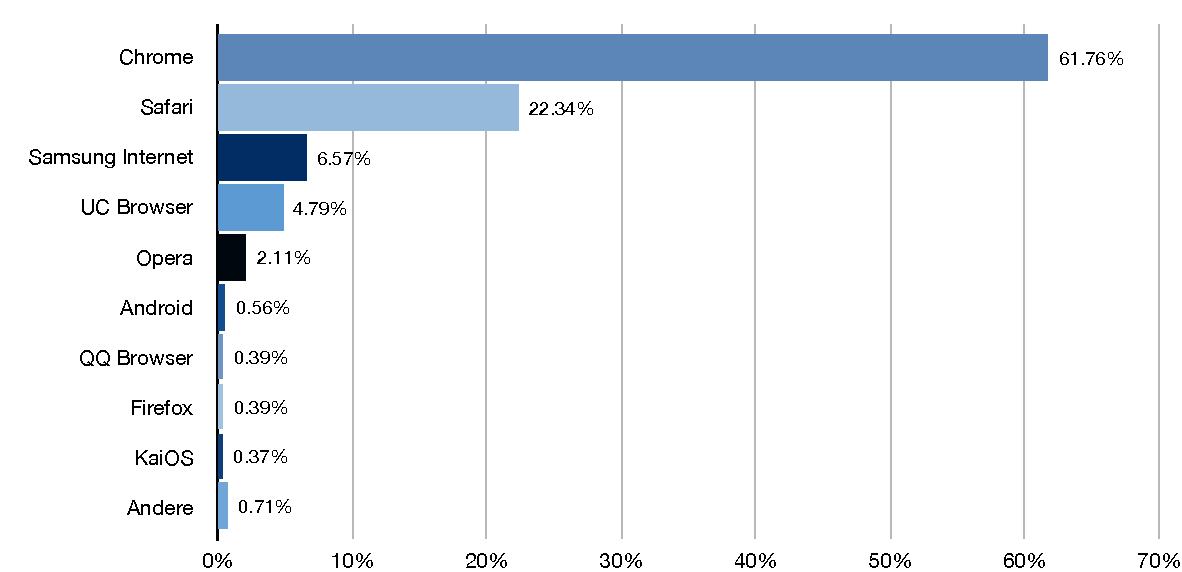
\includegraphics[scale=0.65]{images/browser-market-share}
	\caption{Marktanteile mobiler Browser weltweit (Juni 2019 bis Juli 2020)}
	\label{fig:browser-market-share}
\end{figure}
Der größte Nachteil gegenüber nativen Anwendung ist bis vor einiger Zeit noch die Offlinefähigkeit gewesen. Doch mit dem Ansatz der Progressive Web Apps lassen sich auch Offlinefunktionalitäten mit einbauen. Progressive Web Apps sind webbasierte Anwendungen, welche Offlinefunktionalität bieten und auf native Funktionen, wie Benachrichtigungen und Sensordaten des Gerätes zugreifen können. In sehr spezifischen Anwendungsfällen sind webbasierte Anwendungen nicht geeignet, da die Hersteller der Webbrowser sich nicht alle an die gleichen Standards halten und der Zugriff auf die Hardware über Progressive Web Apps noch eingeschränkt ist \parencite{TOR2020}.

\subsection{Hybride Anwendungen}
Die Herangehensweise der hybriden mobilen Anwendungen versucht die Vorteile aus den nativen und den webbasierten Anwendungen zu vereinen. Eine hybride Anwendung wird mit Webtechnologien (zum Beispiel HTML, CSS und Javascript) entwickelt, da diese nicht an ein Betriebssystem gebunden sind. Anders als bei den webbasierten Anwendungen wird der entwickelte Code in einen Wrapper abgelegt, welcher den Code interpretiert und je nach Betriebssystem auf die entsprechenden nativen Schnittstellen zugreift. Dadurch erhält man eine mit Webtechnologien entwickelte Anwendung, die auf dem Endgerät als native Anwendung läuft und aus den App Stores heruntergeladen werden können \parencite{HUY2017}. Dies kann auch zu Problemem führen, wenn man eine Funktionalität eines Betriebssystems nutzen möchte, die es auf anderen Betriebssystemen nicht gibt. Deshalb kann hybrider Code oft Ausnahmen enthalten, die je Betriebssystem unterschiedliche Funktionen ausführen oder gar enthalen.\pbreak%
%
Für eine Anwendung dieser Art ist es besonders wichtig, dass sie stabil und zuverlässig läuft.
Es sollten keine Fehler beim Zeichnen auf den Kartendaten entstehen, da richtige Koordinaten für ein valides \acl{imdf} ausschlaggebend sind.
Gerade im Hinblick auf das Herauslesen der Koordinaten anhand einer Karte wurde sich dafür entschieden, einen nativen Ansatz zu wählen.
Da das \acl{imdf} ein von Apple spezifizierter Standard ist und das \Gls{sdk} für iOS Werkzeuge bereitstellt dieses Format zu interpretieren, wird die Anwendung für iOS-Geräte entwickelt.
